\chapter{Testing and Continuous Integration}
\label{chapter:testingAndCI}

Implemented functionality should always be tested. Not only to ensure that it does what it is supposed to do, but also to avoid regression. Nothing is worse than introducing a bug by implementing a new feature without noticing it. Therefore, unit, snapshot and end-to-end test are used to avoid regression in this project.
Moreover, all tests are run on each commit to the GitLab repository.

\section{Testing}
\label{section:testing}
For unit and snapshot testing Jest is used. Jest is a JavaScript testing framework focusing on simplicity and is maintained by Facebook. It is supposed to require zero configuration and runs tests isolated and therefore can be parallelized \cite{Jest}. For end-to-end testing Nightwatch is used. Nightwatch is a Node.js powered end-to-end testing framework for web applications. It supports testing in Chrome, Firefox and Edge, has the concept of page objects to easily abstract the content of a page and allows extending the framework with custom commands \cite{Nightwatch}.

\subsection{Unit Testing}
\label{subsection:unitTesting}
Unit tests are used to verify the correctness of individual functions and apply the following concept: the tester has an input to a function and knows what the function should output for this input. The tester then compares the actual output of the function and compares it to the expected output. If those are not the same the test is evaluated as failed, and succeeded otherwise.

There are mainly two different categories of unit tests: black-box and white-box testing.

\subsection*{Back-box and White-box Testing}
Black-box testing is a testing method, where the tester does not know how a feature is implemented, but knows its specification and creates test based on this knowledge. White-box testing on the other hand is a testing method, where the tester does know the implementation of the feature. Usually, both kind of software testing should be used, but since there are no software tester (testers applying black-box testing) involved in this project, only white-box testing is applied \cite{BlackBoxWhiteBoxTesting}.

\subsection*{Test Plan}

General purpose components are tested in its specialized functionality i.e whether they react correctly on different user inputs. 
\TODO{maybe elaborate on that?}
The components representing an exercises are tested for:

\begin{itemize}
    \item Initial conditions hold
    \item Various exercise specific user inputs are handled correctly
    \item Restarting the exercise works as expected
    \item Starting next example restores the initial conditions
    \item Correct answer is accepted
    \item Incorrect answer is rejected
\end{itemize}

\subsection*{Code Coverage}
As mentioned before, unit test usually test a feature on the function level. To catch as many possible code paths and corner cases, the same function is tested multiple times with different inputs. 
A metric to judge the usefulness of a test suite is the code coverage. The code coverage shows how well a test suite covers the functionality. Usually, a coverage report includes:

\begin{itemize}
    \item \textbf{Statement coverage} - The percentage of statements that have been executed 
    \item \textbf{Branch coverage} - The percentage of branches of the control structures (e.g. if and loop statements) that have been executed
    \item \textbf{Function coverage} - The percentage of functions that have been called
    \item \textbf{Lines coverage} - The percentage of line of the source code that have been tested
\end{itemize}

High coverage percentage does not imply that it is a good test suite. Some critical paths can still be untested. It is generally accepted that a code coverage of 80\% is a desirable goal. Going above 80\% of code coverage is usually costly and does not provide any valuable benefit \cite{CodeCoverage}.

The code coverage for the whole project and each component is given in table \ref{table:testCoverage}. Most of the components are well tested with a code coverage of above 80\% in most categories. Some percentages indicate bad code coverage. Usually those components with bad code coverage have less than forty lines and therefore not tested thoroughly. 
 
\subsection*{Non-determinism}
A problem that has to be tackled for testing is how to handle determinism. Some exercises are based on random behaviour to achieve a rich user experience. However, if random behaviour is used, then the actual output may not be the same as the expected output and the test is evaluated as failed. To circumvent this issue, one can mock the function that is used to generate a random numbers. Mock functions allow to overwrite the actual implementation of the function by intercepting calls to this function and return values configured by the test suite \cite{Jest}. 
\TODO{maybe refer to game mixin}

\begin{table}
    \caption{Test coverage of all components}
    \centering
    \begin{tabular}{|l|l|l|l|l|}
    \hline
        File & \% Statements & \% Branches & \% Functions & \% Lines \\ \hline
        All files & 86.71 & 73.11 & 86.73 & 86.56 \\ \hline
        App.vue & 100 & 100 & 100 & 100 \\ \hline
        GameMixins.vue & 55.56 & 100 & 27.27 & 55.56 \\ \hline
        Home.vue & 100 & 100 & 100 & 100 \\ \hline
        ciphertexts/PatternEncryption.vue & 79.41 & 50 & 81.82 & 78.13 \\ \hline
        ciphertexts/PatternDecryption.vue & 78.79 & 50 & 80 & 77.42 \\ \hline
        layout/Footer.vue & 100 & 100 & 100 & 100 \\ \hline
        layout/Header.vue & 100 & 100 & 100 & 100 \\ \hline
        numbersystems/From.vue & 100 & 100 & 100 & 100 \\ \hline
        numbersystems/ItemDropzone.vue & 100 & 100 & 100 & 100 \\ \hline
        numbersystems/ItemGroup.vue & 100 & 100 & 100 & 100 \\ \hline
        numbersystems/NumbersystemsMixin.vue & 75.41 & 62.5 & 84.62 & 77.59 \\ \hline
        numbersystems/Swap.vue & 88.89 & 83.33 & 88.89 & 91.18 \\ \hline
        numbersystems/To.vue & 90.24 & 45.45 & 90 & 92.11 \\ \hline
        shared/Buttonmenu.vue & 66.67 & 100 & 0 & 66.67 \\ \hline
        shared/Difficulty.vue & 87.5 & 62.5 & 100 & 87.5 \\ \hline
        shared/ItemSelection.vue & 100 & 100 & 100 & 100 \\ \hline
        shared/Modal.vue & 100 & 100 & 100 & 100 \\ \hline
        shared/Trashcan.vue & 100 & 100 & 100 & 100 \\ \hline
        shared/Tutorial.vue & 100 & 100 & 100 & 100 \\ \hline
        shared/Undo.vue & 100 & 100 & 100 & 100 \\ \hline
        trees/Row.vue & 89.04 & 65.71 & 100 & 88.89 \\ \hline
        trees/Sudoku.vue & 91.12 & 76.09 & 94.12 & 90.26 \\ \hline
        trees/TreesMixin.vue & 100 & 100 & 100 & 100 \\ \hline
        words/Add.vue & 98.33 & 100 & 95.24 & 98.28 \\ \hline
        words/Change.vue & 91.43 & 83.33 & 93.33 & 91.18 \\ \hline
        words/Remove.vue & 100 & 100 & 100 & 100 \\ \hline
        words/Swap.vue & 61.22 & 87.5 & 76 & 59.78 \\ \hline
    \end{tabular}
    \label{table:testCoverage}
\end{table}

\subsection{Snapshot Testing}
\label{subsection:snapshotTesting}
Snapshot tests ensures correctness of the user interface and that it does not change unexpectedly. More precisely, snapshot tests renders the template of a component to HTML, takes a snapshot and compares the snapshot with the previous saved reference snapshot. These two snapshots are compared and if they do not match, the test fails or succeeds otherwise. If the changes made to the source code were intended to change the UI, the snapshot has to be updated. This requires an initial snapshot that is known to be correct. Hence snapshot should be committed to the repository as well \cite{Jest}.

Every component in this project is snapshot tested and is therefore save from unintended UI changes.

\subsection{End-to-End Testing}
\label{subsection:e2e}
end-to-end tests are used to test the entire application flow through an application. The main goal is to test it from a users perspective by simulating a user scenario \cite{EndToEndTests}. 
\TODO{maybe elaborate a bit more on that}

Nightwatch allows to run end-to-end tests for Chrome, Firefox and Edge to ensure the application works across browser-borders. The end-to-end tests for this project make use of page objects. A page object is an abstraction of a page represented as an object. The goal of a page object is to simplify the end-to-end test by showing the same one can see when one visits the page \cite{Nightwatch}.

The end-to-end tests in this project only covers the visibility of all parts of an exercise one needs to see to solve it. The reason behind this is that many exercises are based on non-determinism and since a user cannot influence that the end-to-end tests are not able to do that as well.

\section{Continuous Integration}
\label{section:CI}

This project make use of the GitLab Continuous Integration (CI). When pushing a commit to the projects GitLab repository, the CI pipeline is run (figure \ref{fig:pipeline}). The CI pipeline is specified in the \code{.gitlab-ci.yml} file in the projects root folder and specifies what jobs need to be done. Usually, these jobs build, test and validate changes made to the source code and allow to easily catch bugs and errors.
The CI pipeline of this project consists of two parts:

\begin{itemize}
    \item \textbf{Unit and Snapshot tests} - runs the unit and snapshot tests as described in \nameref{subsection:unitTesting} and \nameref{subsection:snapshotTesting}
    \item \textbf{End-to-end tests} - runs the end-to-end tests in Firefox as described in \nameref{subsection:e2e}
\end{itemize}

\begin{figure} 
    \centering
    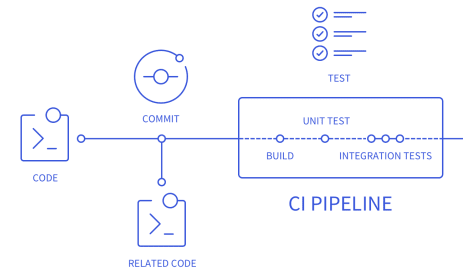
\includegraphics[width=0.6 \columnwidth]{figures/pipeline.png}
    \caption{Pipeline visualization \cite{CIPipeline}} 
    \label{fig:pipeline} 
\end{figure}